\documentclass[10pt]{article}
\usepackage[bottom=1in,left=1in,top=1in,right=0.75in]{geometry}
\usepackage{tabularx}
\usepackage{fancyhdr}
\usepackage{supertabular}
\usepackage{longtable}
\usepackage{makecell}
\usepackage{array}
\usepackage[linkcolor=red,urlcolor=red]{hyperref}
\usepackage[official]{eurosym}
\usepackage[us]{datetime}
\usepackage[pdftex]{graphics}

\setcounter{LTchunksize}{5}

\pagestyle{fancy}
\lhead{(Page \thepage)}
\cfoot{}
\renewcommand{\headrulewidth}{0pt}


\begin{document}

\noindent
\begin{tabularx}{\linewidth}{XX} 
BIO-BIBLIOGRAPHY & \hfill University of California, Santa Barbara \\ \\
 & \hfill June 30, 2021 \\ \\
 Kelly K. Caylor &   \\ 
 Professor III & \\
 Department of Geography & \\
 Bren School of Environmental Science \& Management & \\
 Director of Earth Research Institute & 
 \end{tabularx}

\vspace{1cm}
% Last update filed on October 6, 2018

This update refers to the period July 1, 2018 to June 30, 2021


\vspace{1cm}
\centering {\textbf{ \large Curriculum Vitae}}

\raggedright

\vspace{0.5cm}
\underline{Education}

University of Virginia, Ph.D., Environmental Sciences, 2003

University of Virginia, B.A., with High Distinction, Environmental Sciences, 1996

\vspace{0.5cm}
\underline{Areas of Specialization}

Ecohydrology, Isotope hydrology, Coupled natural-human systems, Environmental sensing.

\vspace{0.5cm}
\underline{Previous Academic or Professional Appointments}
\begin{tabular}{l p{5.5in} }

2005 - 2007 \ \ \ \  & Assistant Professor, Department of Geography, Indiana University \\
2007 - \ \ \ \ & Adjunct Faculty, Department of Geography, Indiana University \\ 
2007 - 2012 \ \ \ \ & Assistant Professor, Dept. of Civil and Environmental Engineering, Princeton University \\
2013 - 2016 & Affiliated Faculty, Dept. of Ecology and Evolutionary Biology, Princeton University \\
2013 - 2016 & Associate Professor, Dept. of Civil and Environmental Engineering, Princeton University \\
2014 - 2016 & Director, Environmental Studies Program, Princeton University \\
2016 - \ \ \ \ & Full Professor, Dept. of Geography, University of California, Santa Barbara \\ 
2016 - \ \ \ \ & Full Professor, Bren School of Environmental Science \& Management, UCSB \\ 

\end{tabular}

\vspace{0.5cm}
\underline{Professional Organizations}

American Geophysical Union, Association of American Geographers, American Association for the Advancement of Science

\vspace{0.5cm}

\newpage

\textbf{PART I.  RESEARCH}

\vspace{0.2cm}
{\bf Cumulative List of Publications (or Creative Activities):}

%\vspace{0.2cm}
{\setlength{\extrarowheight}{3.5pt}
% UC Bio-bib Publication Table
% Created on 2019-11-19 10:42

\begin{longtable}{lcp{7.75cm}>{\raggedright}p{5.25cm}p{1.75cm}}
\# & Year & Title and Authors & Publisher & Category\\
\hline 
\endhead 
    1.0 & 2000 & {\bf Approaches for the estimation of primary productivity and vegetation structure in the Kalahari region }, Dowty, P.R., Caylor, K.K., Shugart, H.H,, Emanuel, W.R. & Ringrose, S., Chanda, R. (eds.). \emph{ Towards Sustainable Natural Resource Management in the Kalahari Region.  }. University of Botswana Press & Refereed Book Chapter\\
    2.0 & 2002 & {\bf The southern African Regional Science Initiative (SAFARI 2000): Wet season campaigns}, Otter, LB, Scholes, RJ, Dowty, PR, Privette, JP, Caylor, K.K., Ringrose, S, Mukelabai, M, Frost, P, Hanan, N, Totolo, O, Veenendall, EM. \href{https://ucsb.box.com/s/b6gdsjokzr9s3c517rc0wzuciokb9ed2}{[pdf]} & \emph{ South African Journal of Science } 98(3-4): 131-137.   & Refereed Article\\
    3.0 & 2002 & {\bf Determining land surface fractional cover from NDVI and rainfall time series for a savanna ecosystem}, Scanlon, TM, Albertson, JD, Caylor, K.K., Williams, CA. \href{https://ucsb.box.com/s/dne61k069ujkhwqno7fyjopjkkaoro0z}{[pdf]} & \emph{ Remote Sensing of Environment } 82(2-3): 376-388. doi:10.1016/s0034-4257(02)00054-8.  & Refereed Article\\
    4.0 & 2002 & {\bf Trends in savanna structure and composition on an aridity gradient in the Kalahari}, Scholes, RJ, Dowty, PR, Caylor, K.K., Parsons, DAB, Frost, PGH, Shugart, HH. \href{https://ucsb.box.com/s/oo1omprvq0s6l8vbnihnc9eot6pk6ej2}{[pdf]} & \emph{ Journal of Vegetation Science } 13(3): 419-428. doi:10.1111/j.1654-1103.2002.tb02066.x.  & Refereed Article\\
    5.0 & 2003 & {\bf Tree spacing along the Kalahari transect in southern Africa}, Caylor, K.K., Shugart, HH, Dowty, PR, Smith, TM. \href{https://ucsb.box.com/s/o5jxbx1brdt7epgfwtmpojfva120mcfm}{[pdf]} & \emph{ Journal of Arid Environments } 54(2): 281-296. doi:10.1006/jare.2002.1090.  & Refereed Article\\
    6.0 & 2003 & {\bf Release of gaseous and particulate carbonaceous compounds from biomass burning during the SAFARI 2000 dry season field campaign}, Hely, C, Caylor, K.K., Alleaume, S, Swap, RJ, Shugart, HH. \href{https://ucsb.box.com/s/jztfplnyhywtwh6ipki4pkcn3txghbro}{[pdf]} & \emph{ Journal of Geophysical Research - Atmospheres } 108(13). doi:10.1029/2002jd002482.  & Refereed Article\\
    7.0 & 2003 & {\bf Regional fuel load for two climatically contrasting years in southern Africa}, Hely, C, Dowty, PR, Alleaume, S, Caylor, K.K., Korontzi, S, Swap, RJ, Shugart, HH, Justice, CO. \href{https://ucsb.box.com/s/36fbprbjg0ba8945fedk5xicnccg4urx}{[pdf]} & \emph{ Journal of Geophysical Research - Atmospheres } 108(13). doi:10.1029/2002jd002341.  & Refereed Article\\
    8.0 & 2003 & {\bf Soil moisture and plant stress dynamics along the Kalahari precipitation gradient}, Porporato, A, Laio, F, Ridolfi, L, Caylor, K.K., Rodriguez-Iturbe, I. \href{https://ucsb.box.com/s/jf70c4uz24j4an6fczk5i4dk4sji2fze}{[pdf]} & \emph{ Journal of Geophysical Research - Atmospheres } 108(D3). doi:10.1029/2002jd002448.  & Refereed Article\\
    9.0 & 2004 & {\bf Coupling ecohydrological patterns and processes in semi-arid landscapes}, Caylor, K.K., Rodriguez-Iturbe, I &  \emph{ Proceedings of the British Hydrological Society's International Conference on Hydrology: Science \& Practice for the 21st Century }. British Hydrological Society & Refereed Conference Proceedings\\
    10.0 & 2004 & {\bf Simulated productivity of heterogeneous patches in Southern African savanna landscapes using a canopy productivity model}, Caylor, K.K., Shugart, HH. \href{https://ucsb.box.com/s/3o5vjkcv360inv882y350su6oj9xiw6d}{[pdf]} & \emph{ Landscape Ecology } 19(4): 401-415. doi:10.1023/B:LAND.0000030450.11302.c2.  & Refereed Article\\
    11.0 & 2004 & {\bf Feasible optimality of vegetation patterns in river basins}, Caylor, K.K., Scanlon, TM, Rodriguez-Iturbe, I. \href{https://ucsb.box.com/s/we0zwbqk1qgsfve671x81gkayzqlgsrj}{[pdf]} & \emph{ Geophysical Research Letters } 31(13). doi:10.1029/2004GL020260.  & Refereed Article\\
    12.0 & 2004 & {\bf Relationship between small-scale structural variability and simulated vegetation productivity across a regional moisture gradient in southern Africa}, Caylor, K.K., Dowty, PR, Shugart, HH, Ringrose, S. \href{https://ucsb.box.com/s/x6m4zd215u3x0b9xcphsrym5m0itb103}{[pdf]} & \emph{ Global Change Biology } 10(3): 374-382. doi:10.1111/j.1365-2486.2003.00704.x.  & Refereed Article\\
    13.0 & 2004 & {\bf Vegetation structure characteristics and relationships of Kalahari woodlands and savannas}, Privette, JP, Tian, Y, Roberts, G, Scholes, RJ, Wang, Y, Caylor, K.K., Mukelabai, M. \href{https://ucsb.box.com/s/9v3epeslmv63b8aro7776cx4miuh7c8p}{[pdf]} & \emph{ Global Change Biology } 10(3): 281-291. doi:10.1111/j.1365-2486.2004.00740.x.  & Refereed Article\\
    14.0 & 2004 & {\bf A  simulation analysis of the detectability of understory burns in miombo woodlands}, Pereira, JMC, Mota, B, Privette, JL, Caylor, K.K., Silva, JMN, Sa, ACL, Ni-Meister, W. \href{https://ucsb.box.com/s/0lzypk2gojo3azveiaxb5ei5sjbrrgzs}{[pdf]} & \emph{ Remote Sensing of Environment } 93(3): 296-310. doi:10.1016/j.rse.2004.01.009.  & Refereed Article\\
    15.0 & 2005 & {\bf Tree canopy effects on simulated water stress in southern African savannas}, Caylor, K.K., Shugart, HH, Rodriguez-Iturbe, I. \href{https://ucsb.box.com/s/6xx8sd7ds9bwjaw5ofjv3p2nqx3nhqnf}{[pdf]} & \emph{ Ecosystems } 8(1): 106-121. doi:10.1007/s10021-004-0027-9.  & Refereed Article\\
    16.0 & 2005 & {\bf On the coupled geomorphological and ecohydrological organization of river basins}, Caylor, K.K., Manfreda, S., Rodriguez-Iturbe, I. \href{https://ucsb.box.com/s/c5rmun9bvc6e62zycsk6tj4yyabrmnd0}{[pdf]} & \emph{ Advances in Water Resources } 28(1): 69-86. doi:10.1016/j.advwatres.2004.08.013.  & Refereed Article\\
    17.0 & 2005 & {\bf Dynamic response of grass cover to rainfall variability: Implications for the function and persistence of savanna ecosystems}, Scanlon, TM, Caylor, K.K., Manfreda, Salvatore, Levin, Simon, Rodriguez-Iturbe, I. \href{https://ucsb.box.com/s/2mlqvq04i8bm5rzct19de60mm08b3nl5}{[pdf]} & \emph{ Advances in Water Resources } 28(3): 291-302. doi:10.1016/j.advwatres.2004.10.014.  & Refereed Article\\
    18.0 & 2005 & {\bf Determinants of woody cover in African savannas: A continental scale analysis}, Sankaran, M, Hanan, N, Scholes, B, Ratnam, Jayashree, 24 others, Caylor, K.K.. \href{https://ucsb.box.com/s/emjsq5yd73cuciidghsf9lyyfyzssdd8}{[pdf]} & \emph{ Nature } 438(7069): 846. doi:10.1038/nature04070.  & Refereed Article\\
    19.0 & 2006 & {\bf Dynamic change in the woodland and savanna ecosystems of sub-tropical Africa. }, Shugart, H.H, Caylor, K.K., Hely, C., Swap, R.J., Dowty, P.R. & Laurence, W., Peres, C. (eds.). \emph{ Emerging Threats to Tropical Forests }. University of Chicago Press & Refereed Book Chapter\\
    20.0 & 2006 & {\bf Pattern and process in savanna ecosystems}, Caylor, K.K, Shugart, H.H. & D'Odorico, P., Porporato, A. (eds.). \emph{ Dryland Ecohydrology }. Springer & Refereed Book Chapter\\
    21.0 & 2006 & {\bf On the ecohydrology of structurally heterogeneous semi-arid landscapes}, Caylor, K.K., D'Odorico, P, Rodriguez-Iturbe, I. \href{https://ucsb.box.com/s/dxwovbqk21d5l7xov1oyv2f1lton0bvu}{[pdf]} & \emph{ Water Resources Research } 42(7). doi:10.1029/2005WR004683.  & Refereed Article\\
    22.0 & 2007 & {\bf Ecohydrological optimization of patterns and processes in water-limited ecosystems.}, Caylor, K.K., Scanlon, T.M., Rodriguez-Iturbe, I. &  \emph{ Water and the Environment: Proceedings of the Workshop in the Vatican Academy of Sciences. }. Vatican Academy of Sciences & Refereed Conference Proceedings\\
    23.0 & 2007 & {\bf A temporal and spatially explicit Production Efficiency Model for fuel load allocation in southern Africa}, Hely, C, Caylor, K.K., Dowty, PR, Alleaume, S, Swap, RJ, Shugart, HH, Justice, CO. \href{https://ucsb.box.com/s/xfohy15ulq1bll4kxxs572z2mdmk2s4n}{[pdf]} & \emph{ Ecosystems } 10(7): 1116. doi:10.1007/s10021-007-9082-3.  & Refereed Article\\
    24.0 & 2007 & {\bf Spatial variation in vegetation structure coupled to plant available water at landscape scales in a Brazilian savanna}, Ferira, J., Bustamente, M, Garcia-Montiel, DC, Caylor, K.K., Davidson, EA. \href{https://ucsb.box.com/s/lr66b9viri9psv6llveasghlfhopni7r}{[pdf]} & \emph{ Oecologia } 153(2): 417-430. doi:10.1007/s00442-007-0747-6.  & Refereed Article\\
    25.0 & 2007 & {\bf When is breeding for drought tolerance optimal when drought is random?}, Sambatti, J, Caylor, K.K.. \href{https://ucsb.box.com/s/3eoevsppc8d3f9rgzs8s84iq6zs1bgu9}{[pdf]} & \emph{ New Phytologist } 175(1): 70-80. doi:10.1111/j.1469-8137.2007.02067.x.  & Refereed Article\\
    26.0 & 2007 & {\bf On soil moisture–vegetation feedbacks and their possible effects on the dynamics of dryland ecosystems}, D'Odorico, P, Caylor, K.K., Okin, GS, Scanlon, TM. \href{https://ucsb.box.com/s/vwn5pfu2jgkou99j85jmsg2vrpw83y3k}{[pdf]} & \emph{ Journal of Geophysical Research - Biogeosciences } 112(G4). doi:10.1029/2006jg000379.  & Refereed Article\\
    27.0 & 2007 & {\bf Positive feedbacks promote power-law clustering of Kalahari vegetation}, Scanlon, TM, Caylor, K.K., Levin, Simon, Rodriguez-Iturbe, I. \href{https://ucsb.box.com/s/7qtnmbzokvw0zkfitybnfgnjrfamy9xi}{[pdf]} & \emph{ Nature } 449(7159): 209. doi:10.1038/nature06060.  & Refereed Article\\
    28.0 & 2008 & {\bf Spatial patterns of soil nutrients in two southern African savannas}, Okin, GS, Mladenov, N, Wang, L, Cassel, D, Caylor, K.K., Ringrose,S. \href{https://ucsb.box.com/s/vwn5pfu2jgkou99j85jmsg2vrpw83y3k}{[pdf]} & \emph{ JGR - Biogeosciences } 113(G2). doi:10.1029/2007JG000584.  & Refereed Article\\
    29.0 & 2009 & {\bf Decoupling structural and environmental determinants of sap velocity}, Dragoni, D., Caylor, K.K. &  \emph{ Proceedings of the 7th International Workshop on Sap Flow, Seville, Spain }. Acta Horticulture & Refereed Conference Proceedings\\
    30.0 & 2009 & {\bf On the calibration of continuous, high-precision $\delta$18O and $\delta$2H measurements using an off-axis integrated cavity output spectrometer }, Wang, L, Caylor, K.K., Dragoni, D.. \href{https://ucsb.box.com/s/jj2w5hte5ylavn9tklog6cwabfjwa8o1}{[pdf]} & \emph{ Rapid Communications in Mass Spectrometry } 23(4): 530-536. doi:10.1002/rcm.3905.  & Refereed Article\\
    31.0 & 2009 & {\bf Ecohydrological optimization of pattern and process in dryland ecosystems: A tradeoff-based hypothesis}, Caylor, K.K., Scanlon, TM, Rodriguez-Iturbe, I. \href{https://ucsb.box.com/s/0di3gazj7qy10ebwrbc5s59di8htc044}{[pdf]} & \emph{ Water Resources Research } 45(8). doi:10.1029/2008WR007230.  & Refereed Article\\
    32.0 & 2009 & {\bf Decoupling structural and environmental determinants of sap velocity: Part II, Observational application}, Dragoni, D, Caylor, K.K., Schmid, H. \href{https://ucsb.box.com/s/tb6bdp2c2rdn0t1rq67hdl8pwqj3m6h1}{[pdf]} & \emph{ Agriculture \& Forest Meteorology } 149(3-4): 570-581. doi:10.1016/j.agrformet.2008.10.006.  & Refereed Article\\
    33.0 & 2009 & {\bf Decoupling structural and environmental determinants of sap velocity: Part I, Methodological development}, Caylor, K.K., Dragoni, D.. \href{https://ucsb.box.com/s/prcsjqnfq5804lswldq6zighqnzkzin2}{[pdf]} & \emph{ Agriculture \& Forest Meteorology } 149(3-4): 559-569. doi:10.1016/j.agrformet.2008.10.010.  & Refereed Article\\
    34.0 & 2009 & {\bf Spatial heterogeneity and sources of soil carbon in Southern African savannas}, Wang, L, Okin, G., Caylor, K.K., Macko, S. \href{https://ucsb.box.com/s/8md68vrqespqol94lfg6qwxfc6al3s49}{[pdf]} & \emph{ Geoderma } 149(3-4): 402-408.   & Refereed Article\\
    35.0 & 2010 & {\bf Combined effect of soil moisture and nitrogen availability variations on grass productivity in African savannas}, Wang, L, D'Odorico, P, Ries, L., Caylor, K.K., Macko, S. \href{https://ucsb.box.com/s/5g5my565pfyu35e7di3nhomo6v9io6hc}{[pdf]} & \emph{ Plant \& Soil } 328(1-2): 95-108. doi:10.1007/s11104-009-0085-z.  & Refereed Article\\
    36.0 & 2010 & {\bf Nutrient limitation on above-ground grass production in four savanna types along the Kalahari Transect}, Ries-O'Halloran, L, Shugart, HH, Wang, L, Caylor, K.K., Ringrose, S. \href{https://ucsb.box.com/s/3kgdtat25d2a83jrww12w41u5k6mxz49}{[pdf]} & \emph{ Journal of Arid Environments } 74(2): 284-290. doi:10.1016/j.jaridenv.2009.08.012.  & Refereed Article\\
    37.0 & 2010 & {\bf An ecohydrological approach to  predict regional species distribution patterns in dryland ecosystems}, Franz, T., Caylor, K.K., Rodriguez-Iturbe, I. , Celia, M., Norbotton, J. \href{https://ucsb.box.com/s/3rtg5n9k01htohse3ek4uqrcjxscjavw}{[pdf]} & \emph{ Advances in Water Resources } 33(2): 215-230. doi:10.1016/j.advwatres.2009.12.003.  & Refereed Article\\
    38.0 & 2010 & {\bf On the importance of accurate depiction of infiltration processes on model soil moisture and vegetation water stress}, Manfreda, S., Scanlon, TM, Caylor, K.K.. \href{https://ucsb.box.com/s/7l91zvvz8qbd3rd18imbdr9cvr5lz579}{[pdf]} & \emph{ Ecohydrology } 3(2): 155-165. doi:10.1002/eco.79.  & Refereed Article\\
    39.0 & 2010 & {\bf Partitioning evapotranspiration across gradients of woody plant cover: assessment of a stable isotope technique}, Wang, L, Caylor, K.K., Villegas, J.C., Barron-Gafford, G, Breshears, DD, Huxman, T. \href{https://ucsb.box.com/s/9goqtpotkkcr8yw0cyvfbfyxuskd81zj}{[pdf]} & \emph{ Geophysical Research Letters } 37(9). doi:10.1029/2010GL043228.  & Refereed Article\\
    40.0 & 2010 & {\bf Herbivores and mutualistic ants interact to regulate tree photosynthesis}, King, E.G., Caylor, K.K.. \href{https://ucsb.box.com/s/dej25f8nw3iiv2t68gvjm3l5lzze6pd6}{[pdf]} & \emph{ New Phytologist } 187(1): 17-21. doi:10.1111/j.1469-8137.2010.03286.x.  & Refereed Article\\
    41.0 & 2011 & {\bf Quantifying Transient Soil Moisture Dynamics Using Multipoint Direct-Current Resistivity in Homogeneous Sand}, Franz, T., Nolan, J, Nordbotten, J, Caylor, K.K., Slater, L.. \href{https://ucsb.box.com/s/67by4alh09ekn109g3f6o7osmako2b44}{[pdf]} & \emph{ Vadose Zone Journal } 10(1): 286-298. doi:10.2136/vzj2010.0031.  & Refereed Article\\
    42.0 & 2011 & {\bf Climatological determinants of woody cover in Africa}, Good, S.P., Caylor, K.K.. \href{https://ucsb.box.com/s/ph7ye2bb98cgnxi09bru3h7u8z7hrad0}{[pdf]} & \emph{ Proceedings of the National Academy of Sciences } 108(12): 4902-4907. doi:10.1073/pnas.1013100108.  & Refereed Article\\
    43.0 & 2011 & {\bf Coupling vegetation organization patterns to soil resource heterogeneity in a central Kenyan dryland using geophysical imagery}, Franz, T., King, E.G., Caylor, K.K., Robinson, DA. \href{https://ucsb.box.com/s/ph7ye2bb98cgnxi09bru3h7u8z7hrad0}{[pdf]} & \emph{ Water Resources Research } 47(7). doi:10.1029/2010WR010127.  & Refereed Article\\
    44.0 & 2011 & {\bf Metabolic principles of river basin organization}, Rodriguez-Itrube, I, Caylor, K.K., Rinaldo, A.. \href{https://ucsb.box.com/s/7cq2hotd50mcsgc36xtjnd4lcwbf4lb9}{[pdf]} & \emph{ Proceedings of the National Academy of Sciences } 108(29): 11751-11755. doi:10.1073/pnas.1107561108.  & Refereed Article\\
    45.0 & 2011 & {\bf Ecohydrology in Practice: Strengths, Conveniences, and Opportunities}, King, E.G., Caylor, K.K.. \href{https://ucsb.box.com/s/akdvjq4ad8xtiawy78c2bamqccaf4hr0}{[pdf]} & \emph{ Ecohydrology } 4(4): 608-612. doi:10.1002/eco.248.  & Refereed Article\\
    46.0 & 2012 & {\bf An ecohydrological approach to predicting hillslope-scale vegetation patterns in dryland ecosystems}, Franz, T., Caylor, K.K., King, E.G., Nordbotten, J, Celia, MA, Rodriguez-Iturbe, I. \href{https://ucsb.box.com/s/klwl8mzwrz5p1xs285tlu0k580iia361}{[pdf]} & \emph{ Water Resources Research } 48(1). doi:10.1029/2011WR010524.  & Refereed Article\\
    47.0 & 2012 & {\bf Multi-sensor derivation of regional vegetation fractional cover in Africa}, Guan, K., Wood, E.F., Caylor, K.K.. \href{https://ucsb.box.com/s/aln8xly7u0z26ysd0vkqc9yx7fgsldni}{[pdf]} & \emph{ Remote Sensing of Environment } 124: 653-665. doi:10.1016/j.rse.2012.06.005.  & Refereed Article\\
    48.0 & 2012 & {\bf Characterizing ecohydrological and biogeochemical connectivity across multiple scales: a new conceptual framework}, Wang, L., Zou, Chris, O'Donnell, F., Good, S., Franz, T., Miller, G.R., Caylor, K.K.. \href{https://ucsb.box.com/s/j7omxu49q6zylp6rfsmackmzsbtf1k1k}{[pdf]} & \emph{ Ecohydrology } 5(2): 221-233. doi:10.1002/eco.1187.  & Refereed Article\\
    49.0 & 2012 & {\bf Ecohydrological interactions in a two-phase mosaic dryland: implications for regime shifts, resilience, and restoration}, King, E.G., Franz, T., Caylor, K.K.. \href{https://ucsb.box.com/s/ycl4jflncrn9jijcposeu7lqp9nhn95b}{[pdf]} & \emph{ Ecohydrology } 5(6): 733-745. doi:10.1002/eco.260.  & Refereed Article\\
    50.0 & 2012 & {\bf Direct quantification of leaf transpiration isotopic composition}, Wang, L, Good, S.P., Caylor, K.K.. \href{https://ucsb.box.com/s/3lmc84h7i6k1t3hu2gi7bojn3aonspga}{[pdf]} & \emph{ Agriculture \& Forest Meteorology } 154: 127-135. doi:10.1016/j.agrformet.2011.10.018.  & Refereed Article\\
    51.0 & 2012 & {\bf A model-based evaluation of woody plant encroachment impacts on coupled carbon and water cycles}, O'Donnell, Caylor, K.K.. \href{https://ucsb.box.com/s/r8w5wjse9tcut4sednns8aplztrw2jcr}{[pdf]} & \emph{ Journal of Geophysical Research - Biogeosciences } 117(G2). doi:10.1029/2011JG001899.  & Refereed Article\\
    52.0 & 2012 & {\bf Understanding the role of ecohydrological feedbacks in ecosystem-state change in drylands}, Turnbull, L, Wilcox, B.P., Belnap, J, Ravi, S, others, Caylor, K.K.. \href{https://ucsb.box.com/s/p3ra3eesr9ri9hbup1ji51zewx973qvt}{[pdf]} & \emph{ Ecohydrology } 5(2): 174-183. doi:10.1002/eco.265.  & Refereed Article\\
    53.0 & 2012 & {\bf Evaluating ecohydrological theories of woody root distribution in the Kalahari}, Bhattachan, A. , Dintwe, K., Tathlego, M., O'Donnell, F., Caylor, K.K., et al.. \href{https://ucsb.box.com/s/pt5mggx0ho7grlm5v3j5q92intkd2bao}{[pdf]} & \emph{ PLoS One } 7(3): e33996. doi:10.1371/journal.pone.0033996.  & Refereed Article\\
    54.0 & 2012 & {\bf Uncertainties in the assessment of the isotopic composition of surface fluxes: A direct comparison of techniques using laser--based water vapor isotope analyzers}, Good, S.P., Soderberg, K., Wang, L, Caylor, K.K.. \href{https://ucsb.box.com/s/l80t1kz9fte7j0f0d0jvf8puvnyje6m2}{[pdf]} & \emph{ Journal of Geophysical Research - Atmospheres } 117(D5). doi:10.1029/2011JD017168.  & Refereed Article\\
    55.0 & 2012 & {\bf Reframing hydrology education to solve coupled human and environmental problems}, King, E.G., O'Donnell, F., Caylor, K.K.. \href{https://ucsb.box.com/s/bgopryyz9x8e7fbq0ysimar5acnfu7c7}{[pdf]} & \emph{ Hydrology and Earth System Science } 16(8): 2293-2404. doi:10.5194/hess-16-4023-2012.  & Refereed Article\\
    56.0 & 2012 & {\bf Stable isotopes of water vapor in the vadose zone: A review of measurement and modeling techniques 
}, Soderberg, K., Good, S.P., Wang, L, Caylor, K.K.. \href{https://ucsb.box.com/s/k197xi9q69aakxc4ujsgyw246hqevtdv}{[pdf]} & \emph{ Vadose Zone Journal } 11(3). doi:10.2136/vzj2011.0165.  & Refereed Article\\
    57.0 & 2012 & {\bf Dryland ecohydrology and climate change: critical issues and technical advances }, Wang, L, D'Odorico, P, Evans, J, Eldridge, T., McCabe, M, Caylor, K.K.. \href{https://ucsb.box.com/s/pkl128akcnquukzrv4nrag63cxctwb1k}{[pdf]} & \emph{ Hydrology and Earth System Science } 16(8): 2585-2603. doi:10.5194/hess-16-2585-2012.  & Refereed Article\\
    58.0 & 2013 & {\bf Seasonal coupling of canopy structure and function in African tropical forests and its environmental controls}, Guan, K., Wolf, A, Medvigy, David, Caylor, K.K., Pan, Ming, Wood, E.F.. \href{https://ucsb.box.com/s/g281d4dvfhe9pdqzjosrdx06vev53ivk}{[pdf]} & \emph{ Ecosphere } 4(3): 1-21. doi:10.1890/ES12-00232.1.  & Refereed Article\\
    59.0 & 2013 & {\bf Using atmospheric trajectories to model the isotopic composition of rainfall in central Kenya}, Soderberg, K., Good, S.P., O'Connor, M, Wang, L, Ryan, K, Caylor, K.K.. \href{https://ucsb.box.com/s/mb6z08pv5zz2vhr9kgvmoufty4vmcmgg}{[pdf]} & \emph{ Ecosphere } 4(3): 1-18. doi:10.1890/ES12-00160.1.  & Refereed Article\\
    60.0 & 2013 & {\bf Ecosystem-scale spatial heterogeneity of stable isotopes of soil nitrogen in African savannas}, Wang, L., Okin, GS, D'Odorico, P, Caylor, K.K., Macko, S. \href{https://ucsb.box.com/s/c1absct28vgn7me40ivbz3wxks2f4w2l}{[pdf]} & \emph{ Landscape Ecology } 28(4): 685-698. doi:10.1007/s10980-012-9776-6.  & Refereed Article\\
    61.0 & 2013 & {\bf The effect of warming on grassland evapotranspiration partition using laser-based isotope monitoring techniques}, Wang, L, Nui, S., Good, S.P., Soderberg, K, others, Caylor, K.K.. \href{https://ucsb.box.com/s/c1absct28vgn7me40ivbz3wxks2f4w2l}{[pdf]} & \emph{ Geochemica et Cosmochimica Acta } 111: 28-38. doi:10.1016/j.gca.2012.12.047.  & Refereed Article\\
    62.0 & 2013 & {\bf Analytical expressions of variability in ecosystem structure and function obtained from three-dimensional stochastic vegetation modelling}, Good, S.P., Rodriguez-Iturbe, I, Caylor, K.K.. \href{https://ucsb.box.com/s/oha7oqh6jmcph7spiqcludn7f291asqi}{[pdf]} & \emph{ Proceedings of the Royal Society, Series A } 469(2155): 20130003. doi:10.1098/rspa.2013.0003.  & Refereed Article\\
    63.0 & 2013 & {\bf Virtual water trade and development in Africa}, Konar, M, Caylor, K.K.. \href{https://ucsb.box.com/s/90cey1mo6xijyv8ofwgq9g18set34zmk}{[pdf]} & \emph{ Hydrology and Earth System Science } 17(10): 3969-3982. doi:10.5194/hess-17-3969-2013.  & Refereed Article\\
    64.0 & 2013 & {\bf On The Vulnerability of Water Limited Ecosystems to Climate Change}, Manfreda, S., Caylor, K.K.. \href{https://ucsb.box.com/s/2gwcpop1y7tla777rrx5jk21wlh77520}{[pdf]} & \emph{ Water } 5(2): 819-833. doi:10.3390/w5020819.  & Refereed Article\\
    65.0 & 2014 & {\bf Multilevel governance of irrigation systems and adaptation to climate change in Kenya }, Dell'Angelo, J, McCord, P.F., Baldwin, E., Cox, M.E., Gower, D., Caylor, K.K., Evans, T.P. & Bhaduri, A., Bogardi, J., Leentvaar, J., Marx, S. (eds.). \emph{ The Global Water System in the Anthropocene }. Springer International & Refereed Book Chapter\\
    66.0 & 2014 & {\bf Integrating short- and long-range processes into models: The emergence of pattern}, Caylor, K.K, Okin, G.S., Turnbull, L., Wainwright, J., Wiegand, T., Franz, T.E., Parsons, A.J. & Mueller, E.N., Wainwright, J., Parsons, A.J., Turnbull, L. (eds.). \emph{ Patterns of Land Degradation in Drylands }. Springer International & Refereed Book Chapter\\
    67.0 & 2014 & {\bf An analysis of structure: biomass structure relationships for characteristic species of the western Kalahari, Botswana}, Meyer, T, D'Odorico, P, Okin, GS, Shugart, HH, Caylor, K.K., O'Donnell FC. \href{https://ucsb.box.com/s/bsay0vhcvkmlhl04pdl7t687eflb2jlm}{[pdf]} & \emph{ African Journal of Ecology } 52(1): 20-29. doi:10.1111/aje.12086.  & Refereed Article\\
    68.0 & 2014 & {\bf $\delta$2H Isotopic flux partitioning of evapotranspiration over a grass field following a water pulse and subsequent dry down}, Good, S.P., Soderberg, K., Guan K., King, E.G., Scanlon, TM, Caylor, K.K.. \href{https://ucsb.box.com/s/tpllvj83demjut0j70vfmrky9ag5g6yh}{[pdf]} & \emph{ Water Resources Research } 50(2): 1410-1432. doi:10.1002/2013WR014333.  & Refereed Article\\
    69.0 & 2014 & {\bf Modelling vegetation patterns in semiarid environments}, Manfreda, S., Pizzolla, T., Caylor, K.K..  & \emph{ Procedia Environmental Sciences } 19: 168-177. doi:10.1016/j.proenv.2013.06.019.  & Refereed Article\\
    70.0 & 2014 & {\bf Deriving vegetation phenological time and trajectory information over Africa using SEVIRI daily LAI}, Guan, K., Medvigy, D., Wood, E.F., Caylor, K.K., Li, S., Jeong, S.. \href{https://ucsb.box.com/s/plw1e6wcw9lncwww0464puen7f83fgzx }{[pdf]} & \emph{ IEEE Transactions on Geoscience and Remote Sensing } 52(2): 1113-1130. doi:10.1109/TGRS.2013.2247611.  & Refereed Article\\
    71.0 & 2014 & {\bf Continental-scale impacts of intra-seasonal rainfall variability on simulated ecosystem responses in Africa}, Guan, K., Good, S.P., Caylor, K.K., Sato, Hisashui, Li, Haibin, Wood, E.F.. \href{https://ucsb.box.com/s/fhm9hn0fzw60fvm9ou7h8pduiunlf0um}{[pdf]} & \emph{ Biogeosciences } 11(23): 6939-6954. doi:10.5194/bg-11-6939-2014.  & Refereed Article\\
    72.0 & 2014 & {\bf Changing water availability during the African maize-growing season, 1979-2010}, Estes, L, Chaney, N., Herrera-Estrada, J., Sheffield, J, Caylor, K.K., Wood, E.F.. \href{https://ucsb.box.com/s/nifv0mfgu42no30r47f9k6mqg5mm1tts}{[pdf]} & \emph{ Environmental Research Letters } 9(7): 75005. doi:10.1088/1748-9326/9/7/075005.  & Refereed Article\\
    73.0 & 2014 & {\bf Global synthesis of vegetation control on evapotranspiration partitioning}, Wang, L., Good, S.P., Caylor, K.K., `. \href{https://ucsb.box.com/s/r5gbwjuynwn6fw8x7cd0452g4jznxfn2}{[pdf]} & \emph{ Geophysical Research Letters } 41(19): 6753-6757. doi:10.1002/2014GL061439.  & Refereed Article\\
    74.0 & 2014 & {\bf Terrestrial hydrological controls on land surface phenology of African savannas and woodlands}, Guan, K., Wood, E.F, Medvigy, D., Wolf, A., Kimball, J., Pan, M., Caylor, K.K., Sheffield, J. \href{https://ucsb.box.com/s/ib8uckd0g1z20jt4jdtry5z2f3yarjy8}{[pdf]} & \emph{ Journal of Geophysical Research - Biogeosciences } 119(8): 1652-1669. doi:10.1002/2013JG002572.  & Refereed Article\\
    75.0 & 2015 & {\bf Photosynthetic seasonality of global tropical forests constrained by hydroclimate}, Guan, K., Pan, M., Li, H., Wolf, A, Medvigy, D, Caylor, K.K., Sheffield, J, Wood, EF, Mahli, Y, Liang, M., others. \href{https://ucsb.box.com/s/9ycpfurog15j1632gjmn4th9uim7c4dl}{[pdf]} & \emph{ Nature Geoscience } 8(4): 284. doi:10.1038/ngeo2382.  & Refereed Article\\
    76.0 & 2015 & {\bf Termite mounds can increase the robustness of dryland ecosystems to climatic change}, Bonachela, J.A., Pringle, RM, Shefer, E, Coverdale, TC, Guyon, JA, Caylor, K.K., Levin, SA, Tarnita, CE. \href{https://ucsb.box.com/s/v8812382lomed561t7tqpsc235lq7xpm}{[pdf]} & \emph{ Science } 347 6222): 651-655. doi:10.1126/science.1261487.  & Refereed Article\\
    77.0 & 2015 & {\bf Carbon stable isotopes suggest that hippopotamus-vectored nutrients subsidize aquatic consumers in an East African river}, McCauley, D.J., Dawson, T, Power, ME, Finlay, JC, Ogada, M, Gower, D., Caylor, K.K.. \href{https://ucsb.box.com/s/plw1e6wcw9lncwww0464puen7f83fgzx}{[pdf]} & \emph{ Ecosphere } 6(4): 1-11. doi:10.1890/ES14-00514.1.  & Refereed Article\\
    78.0 & 2015 & {\bf A quantitative description of the interspecies diversity of belowground structure in savanna woody plants}, O'Donnell, F., Caylor, K.K., Bhattachan, A, Dintwe, Kebonye, D'Odorico, P, Okin, G. \href{https://ucsb.box.com/s/ukycth00kvuyf437bzgij47llr5t2v1t}{[pdf]} & \emph{ Ecosphere } 6(9): 1-15. doi:10.1890/ES14-00310.1.  & Refereed Article\\
    79.0 & 2015 & {\bf Dynamic interactions of ecohydrological and biogeochemical processes in water-limited systems}, Wang, L., Manzoni, S., Ravi, S., Riveros-Iregui, D., Caylor, K.K.. \href{https://ucsb.box.com/s/2bx2kijusjv66z2rjtniu1ob7797htd9}{[pdf]} & \emph{ Ecosphere } 6(8): 1-27. doi:10.1890/ES15-00122.1.  & Refereed Article\\
    80.0 & 2015 & {\bf Warmer and wetter soil stimulates assimilation more than respiration in rainfed agricultural ecosystem on the China Loess Plateau: the role of partially plastic film mulching tillage}, Gong, D., Hao, W., Mei, X., Gao, X., Caylor, K.K.. \href{https://ucsb.box.com/s/bbaob5ga0fva4mmaby17wk27h12ugp3s}{[pdf]} & \emph{ PLoS One } 10(8): e0136578. doi:10.1371/journal.pone.0136578.  & Refereed Article\\
    81.0 & 2015 & {\bf Soil organic C and total N pools in the Kalahari: potential impacts of climate change on C sequestration in savannas}, Dintwe, K., Okin, GS, D'Odorico, P, Hrast, T, Mladenov,N., Handorean, A., Bhattachan, A., Caylor, K.K.. \href{https://ucsb.box.com/s/ux5h1cfgl0wtt1i697t282s1cyg1cxi3}{[pdf]} & \emph{ Plant \& Soil } 396(1-2): 27-44. doi:10.1007/s11104-014-2292-5.  & Refereed Article\\
    82.0 & 2016 & {\bf Global Patterns of the Contributions of Storm Frequency, Intensity, and Seasonality to Interannual Variability of Precipitation}, Good, S.P., Guan, K., Caylor, K.K.. \href{https://ucsb.box.com/s/ux5h1cfgl0wtt1i697t282s1cyg1cxi3}{[pdf]} & \emph{ Journal of Climate } 29(1): 3-15. doi:10.1175/JCLI-D-14-00653.1.  & Refereed Article\\
    83.0 & 2016 & {\bf Improved removal of volatile organic compounds for laser-based spectroscopy of water isotopes.}, Chang, E., Wolf, A., Gerlein-Safdi, C., Caylor, K.K.. \href{https://ucsb.box.com/s/cj7itvayum95iwuvcs0a9qmauerkmlo1}{[pdf]} & \emph{ Rapid Communications in Mass Spectrometry } 30(6): 784-790. doi:doi.org/10.1002/rcm.7497.  & Refereed Article\\
    84.0 & 2016 & {\bf Community Water Governance on Mount Kenya: An Assessment Based on Ostrom's Design Principles of Natural Resource Management}, Dell'Angelo, J, McCord, P, Gower, D., Carpenter, S., Caylor, K., Evans, T.P.. \href{https://ucsb.box.com/s/121sxarla5txswqnswj0qjohygz4sfou}{[pdf]} & \emph{ Mountain Research \& Development } 36(1): 102-115. doi:10.1659/MRD-JOURNAL-D-15-00040.1.  & Refereed Article\\
    85.0 & 2016 & {\bf A platform for crowdsourcing the creation of representative, accurate landcover maps}, Estes, L, McRitchie, D., Choi, J., Debats, S., Evans, T., Guthe, W., Luo, D., Ragazzo, G., Zempleni, R., Caylor, K.K.. \href{https://ucsb.box.com/s/la0w2gbatioro0cwau1hhqohv48evcgy}{[pdf]} & \emph{ Environmental Modelling \& Software } 80: 41-53. doi:10.1016/j.envsoft.2016.01.011.  & Refereed Article\\
    86.0 & 2016 & {\bf A generalized computer vision approach to mapping crop fields in heterogeneous agricultural landscapes}, Debats, S., Luo, D., Estes, L.D., Fuchs, T., Caylor, K.K.. \href{https://ucsb.box.com/s/k2wopfl2eie8q1ebhtfsnzahjshdzty7}{[pdf]} & \emph{ Remote Sensing of Environment } 179: 210-221. doi:10.1016/j.rse.2016.03.010.  & Refereed Article\\
    87.0 & 2016 & {\bf Explaining inter-annual variability of gross primary productivity from plant phenology and physiology}, Zhou, S, Zhang, Y., Caylor, K.K., Luo, Y., Xiao, X., Ciais, P., Huang, Y., Wang, G.. \href{https://ucsb.box.com/s/dkdthi1g8ei5z7e3qeywpeptpdqhy7zf}{[pdf]} & \emph{ Agricultural \& Forest Meteorology } 226: 246-256. doi:10.1016/j.agrformet.2016.06.010.  & Refereed Article\\
    88.0 & 2016 & {\bf Reconciling agriculture, carbon and biodiversity in a savanna transformation frontier}, Estes, L., Searchinger, T., Spiegel, M., Tian, D., Sichinga, S., Mwale, M., Kehoe, L., Kuemmerle, T., Berven, A., Chaney, N., Sheffield, J., Wood, E.F., Caylor, K.K.. \href{https://ucsb.box.com/s/7y17t8cy5s6mzfify64sa091m3h52sm3}{[pdf]} & \emph{ Philosophical Transactions of the Royal Society B - Biological Sciences } 371(1703): 20150316. doi:10.1098/rstb.2015.0316.  & Refereed Article\\
    89.0 & 2016 & {\bf Modeling ecohydrological dynamics of smallholder strategies for food production in dryland agricultural systems}, Gower, D. B., Dell'Angelo, J., McCord, P.F., Caylor, K.K., Evans, T.P.. \href{https://ucsb.box.com/s/jqv8hzzknadrccf4fewcygzu7u6u4eln}{[pdf]} & \emph{ Environmental Research Letters } 11(11): 115005. doi:10.1088/1748-9326/11/11/115005.  & Refereed Article\\
    90.0 & 2017 & {\bf An Ecohydrological Framework to Explain Shifts in Vegetation Organization Across Climatological Gradients}, Manfreda, S., Caylor, K.K., Good, S.P.. \href{https://ucsb.box.com/s/867yn9h3kkytmh21v9t7zkk99nmovynx}{[pdf]} & \emph{ Ecohydrology } 10(3): e1809. doi:10.1002/eco.1809 .  & Refereed Article\\
    91.0 & 2017 & {\bf Dominant role of plant physiology in trend and variability of gross primary productivity in North America}, Zhou, S, Zhang, Y., Ciais, P, Xiao, X.M., Luo, Y.Q., Caylor, K.K., Huang, Y., Wang, G.. \href{https://ucsb.box.com/s/f92ypptz914zwdzu4ayvkv7s3ucmev0o}{[pdf]} & \emph{ Scientific Reports } 7: 41366. doi:10.1038/srep41366.  & Refereed Article\\
    92.0 & 2017 & {\bf Comparison of multi-level water use efficiency between plastic film partially mulched and non-mulched croplands at eastern Loess Plateau of China}, Gong, D., Mei, X., Hao, W., Caylor, K.K.. \href{https://ucsb.box.com/s/a2y6j0bqcsbap97vso87nsb69xs594hb}{[pdf]} & \emph{ Agricultural Water Management } 179: 215-226. doi:10.1016/j.agwat.2016.06.006.  & Refereed Article\\
    93.0 & 2017 & {\bf Household-level heterogeneity of water resources within common-pool resource systems}, McCord, P., Dell'Angelo, J., Gower, D., Caylor, K.K., Evans, T.. \href{https://ucsb.box.com/s/uhbkugiej9ahcf5yxmdc2m93y55n63ts}{[pdf]} & \emph{ Ecology \& Society } 22(1). doi:10.5751/ES-09156-220148.  & Refereed Article\\
    94.0 & 2017 & {\bf Comparison of ET partitioning and crop coefficients between partial plastic mulched and non-mulched maize fields}, Gong, D., Mei, X., Hao, W., Wang, H., Caylor, K.K.. \href{https://ucsb.box.com/s/vzrrbi417and6fo5ke33v65mgwbtpkvj}{[pdf]} & \emph{ Agricultural Water Management } 181: 23-34. doi:10.1016/j.agwat.2016.11.016.  & Refereed Article\\
    95.0 & 2017 & {\bf Triple oxygen isotope composition of leaf waters in Mpala, central Kenya}, Li, S., Levin, N., Soderberg, K, Dennis, K.J., Caylor, K.K.. \href{https://ucsb.box.com/s/hl5lqz12jmsb5nsoyd22sb8avtjj11m9}{[pdf]} & \emph{ Earth \& Planetary Science Letters } 468: 38-50. doi:10.1016/j.epsl.2017.02.015.  & Refereed Article\\
    96.0 & 2017 & {\bf Validation of SMAP surface soil moisture products with core validation sites}, Colliander, A, Jackson, TJ, Bindish, R., others, including, Caylor, K.K.. \href{https://ucsb.box.com/s/7q3rg7qjavmnwvpi9qywmdj0dgj3ao9a}{[pdf]} & \emph{ Remote Sensing of Environment } 191: 215-231. doi:10.1016/j.rse.2017.01.021.  & Refereed Article\\
    97.0 & 2017 & {\bf Leaf water 18O and 2H maps show directional enrichment discrepancy in Colocasia esculenta}, Gerlein-Safdi, C., Gauthier, P., Sinkler, C., Caylor, K.K.. \href{https://ucsb.box.com/s/q6mip5kpmp1k95b30bs0kq19hrsn80do}{[pdf]} & \emph{ Plant, Cell, \& Environment } 40(10): 2095-2108. doi:10.1111/pce.13002.  & Refereed Article\\
    98.0 & 2017 & {\bf Calibration of a parsimonious distributed ecohydrological daily model in a data-scarce basin using exclusively the spatio-temporal variation of NDVI}, Ruiz-Perez, G., Kock, J., Manfreda, Salvatore, Caylor, K.K., Frances, F.. \href{https://ucsb.box.com/s/a6cb8weu9mzhijmmn04ncso1ptobkb4f}{[pdf]} & \emph{ Hydrology and Earth System Science } 21(12): 6235-6251. doi:10.5194/hess-21-6235-2017.  & Refereed Article\\
    99.0 & 2018 & {\bf Simulated sensitivity of African terrestrial ecosystem photosynthesis to rainfall frequency, intensity, and rainy season length}, Guan, K., Good, S.P., Caylor, K.K., Medvigy, D., Pan, Ming, Wood, E.F., Sato, H., Biasutti, M., Chen, M., Ahlstrom, A., Xiangtao, X.. \href{https://ucsb.box.com/s/fxgt9q4iyymow014gkmlzv7seoef405i}{[pdf]} & \emph{ Environmental Research Letters } 13(2): 25013. doi:10.1088/1748-9326/aa9f30.  & Refereed Article\\
    100.0 & 2018 & {\bf Measurements and Observations in the XXI century (MOXXI): innovation and multidisciplinarity to sense the hydrological cycle}, Flavia, T., Selker, J., van de Giesen, N., Abrate, T., Uijlenhoet, R., Porfiri, M., Manfreda, S., Caylor, K.K., 22 others. \href{https://ucsb.box.com/s/3xkyj5wzqlygbp8rl0g8v7krjfjaet3s}{[pdf]} & \emph{ Hydrological Sciences Journal } 63(2): 169-196. doi:10.1080/02626667.2017.1420191.  & Refereed Article\\
    101.0 & 2018 & {\bf A large--area, spatially continuous assessment of land cover map error and its impact on downstream analyses}, Estes, L, Chen, P., Debats, S., Evans, T., Ferreira, S., Kuemmerle, T., Ragazzo, G., Sheffield, J, Wolf, A., Wood, E.F., Caylor, K.K.. \href{https://ucsb.box.com/s/lmpa5jeafcemqzs2tywv10onhw2swd3b}{[pdf]} & \emph{ Global Change Biology } 24(1): 322-337. doi:10.1111/gcb.13904.  & Refereed Article\\
    102.0 & 2018 & {\bf The Spatial and Temporal Domains of Modern Ecology}, Estes, L, Elsen, P., Truer, T., Ahmed, L., Caylor, K.K.., Chang, J., Choi, J., Ellis, E. \href{https://ucsb.box.com/s/vqk744sdw8br130o8xrmkgnycg2gzljm}{[pdf]} & \emph{ Nature Ecology \& Evolution } 2(5): 819. doi:10.1038/s41559-018-0524-4.  & Refereed Article\\
    103.0 & 2018 & {\bf On the Use of Unmanned Aerial Systems for Environmental Monitoring}, Manfreda, S., McCabe, M, Miller, P., Lucas, R., Madrigal, V.P., Mallinis, G., Ben Dor, E., Helman, D., Estes, L., Ciraolo, G., 13 others including Caylor, K.. \href{https://ucsb.box.com/s/eysl21s5luo5jtmd9l367jb6zjj5h0do}{[pdf]} & \emph{ Remote Sensing } 10(4): 641. doi:10.3390/rs10040641.  & Refereed Article\\
    104.0 & 2018 & {\bf Dew-induced transpiration suppression impacts the water and isotope balances of Colocasialeave}, Gerlain-Safdi, C., Gauthier, P.G., Caylor, K.K.. \href{https://ucsb.box.com/s/vo5dtxla6nrkz2rfo4b1sbbx809li6tk}{[pdf]} & \emph{ Oecologia } 187(4): 1041-1051. doi:10.1007/s00442-018-4199-y.  & Refereed Article\\
    105.0 & 2018 & {\bf Dew deposition suppresses transpiration and carbon uptake in leaves}, Gerlain-Safdi, C., Koohafkan, MC, Chung, M., Thompson, S, Rockwell, FE, Caylor, K.K.. \href{https://ucsb.box.com/s/6v2kks339czfpp06xulu1ytgjyw4oon9}{[pdf]} & \emph{ Agriculture \& Forest Meteorology } 259: 305-316. doi:10.1016/j.agrformet.2018.05.015.  & Refereed Article\\
    106.0 & 2018 & {\bf Comparing empirical and survey-based yield forecasts in a dryland agro-ecosystem}, Zhao, Y., Vergopolan, N., Baylis, K, Blekking, J. , Caylor, K.K., Evans, T.P., Giroux, S., Sheffield, J, Estes, L.. \href{https://ucsb.box.com/s/jikwk9vwt8c25xq1cr324dnw9yxcuan1}{[pdf]} & \emph{ Agricultural \& Forest Meteorology } 259: 305-316. doi:10.1016/j.agrformet.2018.06.024.  & Refereed Article\\
    107.0 & 2019 & {\bf Biophysical effects on soil crack morphology in a faunally active dryland vertisol}, DeCarlo, K., Caylor, K.K.. \href{https://ucsb.box.com/s/o7utttzbt5dt04rgopi7l5yhkqepw5bz}{[pdf]} & \emph{ Geoderma } 334: 134-145. doi:10.1016/j.geoderma.2018.07.042.  & Refereed Article\\
    108.0 & 2018 & {\bf A global database of water vapor isotopes measured with high temporal resolution infrared laser spectroscopy}, Wei, Zhongwang, Lee, Xuhui, Aemisegger, Franziska, Benetti, Marion, Berkelhammer, Max, Casado, Mathieu, Caylor, K.K., Christner, E., Dryoff, C., Garcia, O.E., 16 others. \href{https://ucsb.box.com/s/6dlkh6re66gagi6ev0snmrzbltz0m03b}{[pdf]} & \emph{ Scientific Data } . doi:10.1038/sdata.2018.302.  & Refereed Article\\
    109.0 & 2019 & {\bf Cognitive biases about climate variability in smallholder farming systems in Zambia}, Waldman, K, Vergopolan, N., Estes, L.D., Attari, S.Z., Sheffiled, J., Caylor, K.K., Evans, T.P. \href{https://ucsb.box.com/s/g4vig4zzrwlt5jwu3sk3m4p5gkvrm8x2}{[pdf]} & \emph{ Weather, Climate \& Society } . doi:10.1175/WCAS-D-18-0050.1.  & Refereed Article\\
    110.0 & 2019 & {\bf A high-frequency mobile phone data collection approach for research in social-environmental systems: Applications in climate variability and food security in sub-Saharan Africa.}, Giroux, S., Caylor, K.K., Kouper, I., Estes, L., Schumacher, J., Waldman, K., Evans, T..  & \emph{ Environmental Modelling \& Software } . doi:10.1016/j.envsoft.2019.05.011.  & Refereed Article\\
    111.0 & 2019 & {\bf The salience of climate change in farmer decision making within smallholder semi-arid agroecosystems}, Waldman, K, Attari, S, Gower, D, Giroux, S, Evans, T, Caylor, K.K..  & \emph{ Climatic Change } .   & Refereed Article\\
    112.0 & 2019 & {\bf Variability in urban population distributions across Africa}, Tuholske, C., Caylor, K.K., Evans, T., Avery, R..  & \emph{ Environmental Research Letters } . doi:10.1088/1748-9326/ab2432.  & Refereed Article\\
\\hline
\\hline
   &   & {\bf Since Appointment:} &    &   \\\\
\end{longtable}
 % modified to include url to pdf instead of doi for since last review -- argh
}

\vspace{0.2cm}
{\bf Works In Press:}

%\vspace{0.15cm}
{\setlength{\extrarowheight}{3.5pt}
% UC Bio-bib Publications In Press Table
% Created on 2018-06-30 11:35

\tablehead{\# & Year & Title and Authors & Publisher & Category\\ \hline}
\begin{supertabular}{lcp{8.25cm}p{4.75cm}p{1.75cm}}
P-1 & 2018 & {\bf Comparing empirical and survey-based yield forecasts in a dryland agro-ecosystem}, Zhao, Y., Vergopolan, N., Baylis, K, Blekkin, J. , Caylor, KK, Evans, T.P., Giroux, S., Sheffield, J, Estes, L.  & \emph{ Agricultural \& Forest Meteorology } & Refereed Article\\
P-2 & 2018 & {\bf Dew-induced transpiration suppression impacts the water and isotope balances of Colocasialeave}, Gerlain-Safdi, C., Gauthier, P.G., Caylor, KK  & \emph{ Oecologia } & Refereed Article\\
\end{supertabular}


}

 

\vspace{0.2cm}

{\bf Work Submitted:}

% For some reason, I need this for the list to appear...
% {\tiny :}

% %\vspace{0.15cm}
% {\setlength{\extrarowheight}{3.5pt}
% % UC Bio-bib Publications Submitted Table
% Created on 2018-10-10 23:23

\begin{longtable}{lcp{7.75cm}>{\raggedright}p{5.25cm}p{1.75cm}}
\# & Year & Title and Authors & Publisher & Category\\
\hline 
\endhead 
C-1 & 2018 & {\bf Changes of daily evapotranspiration partitioning and  water use efficiency with a soil wetting-drying cycle in a sprinkle-irrigated cropland}, Xurong, M., Gong, D., Heng, L., Hsiao, T., Hao, W., Guo, Z., Li, Y, Caylor, K.K..  & \emph{ Science of the Total Environment } .   & Refereed Article\\
C-2 & 2018 & {\bf Labor Sharing and Community-Level Vulnerability to Drought}, Schmitt-Harsh, M, Sweeney, S., Estes, L., Caylor, K.K., Evans, T..  & \emph{ World Development } .   & Refereed Article\\
C-3 & 2018 & {\bf Mapping cropland in an smallholder-dominated African savannas biome using spectral mixture analysis and binary logistic regression}, Sweeney, S, Ruseva, T., Estes, L, Caylor, K.K., Evans, T..  & \emph{ Remote Sensing of Environment } .   & Refereed Article\\
C-4 & 2018 & {\bf The Relative Influences of Climate and Crop Subsidies in Shaping Agricultural Land Use and Productivity}, Mastrorillo, M, Vink, N., Caylor. K., Oppenheimer, M., Estes, L..  & \emph{ Environmental Research Letters } .   & Refereed Article\\
C-5 & 2018 & {\bf The salience of climate change in farmer decision making within smallholder semi-arid agroecosystems}, Waldman, K, Attari, S, Gower, D, Giroux, S, Evans, T, Caylor, K.K..  & \emph{ Climatic Change } .   & Refereed Article\\
C-6 & 2018 & {\bf Perceptions and biases about climate variability in smallholder farming systems}, Waldman, K, Vergopolan, N., Attari, S.Z., Sheffiled, J., Estes, L.D., Caylor, K.K., Evans, T.P.  & \emph{ Weather \& Society } .   & Refereed Article\\
C-7 & 2018 & {\bf A high-frequency mobile phone data collection approach for research in social-environmental systems: Applications in climate variability and food security in sub-Saharan Africa.}, Giroux, S., Caylor, K.K., Kouper, I., Estes, L., Schumacher, J., Waldman, K., Evans, T..  & \emph{ Environmental Modelling \& Software } .   & Refereed Article\\
C-8 & 2018 & {\bf A global database of water vapor isotopes measured with high temporal resolution infrared laser spectroscopy}, Wei, Zhongwang, Lee, Xuhui, Aemisegger, Franziska, Benetti, Marion, Berkelhammer, Max, Casado, Mathieu, Caylor, K.K., Chrsiner, Emanuel, Dryoff, Christoph, Garcia, O.E., 17 others.  & \emph{ Scientific Data } .   & Refereed Article\\
\end{longtable}


% }
None Provided.


\vspace{1cm}
\textbf{PART II.  TEACHING (50\% Geography Dept. workload; 50\% Bren School workload. 50\% Administrative teaching release throughout the review period.)}

\vspace{0.5cm}

\textbf{Workload Descriptions}

\begin{enumerate}
{\footnotesize

\item {\em Geography Department}: Geography department teaching workload for full-time ladder faculty is 3 Instructional Workload Courses (IWC) per year. 50\% workload is 1.5 IWC per year.

\item {\em Bren School}:  The official teaching workload in the Bren School for full-time ladder faculty members is 3.5 Instructional Workload Courses (IWC) per academic year. Full-time faculty are expected to be in residence during the academic year and teach at least two out of three quarters unless they are on sabbatical or approved leave. Each quarter on sabbatical counts as 1.17 IWC for full-time faculty. The teaching workload for faculty with partial appointments is the equivalent fraction of 3.5 and the teaching workload is negotiated with the dean. 50\% workload is 1.75 IWC per year.

Every full-time faculty member will advise or co-advise a Master’s Group Project (ESM 401 series) or Eco-E Project (ESM 402 series) equivalent to 1 IWC. Faculty advisors are expected to meet with master’s groups weekly during the academic year.

Course Equivalencies:
\begin{itemize}
    \item ESM 401A/ESM 402A: 4 units = 0.29 IWC 
    \item ESM 401B/ESM 402B: 4 units = 0.29 IWC
    \item ESM 401C/ESM 402C: 4 units = 0.29 IWC
    \item ESM 401D/ESM 402D: 2 units = 0.13 IWC
\end{itemize}

Every full-time faculty member will teach and/or co-teach core courses, elective courses and seminars in the MESM and PhD programs equivalent to at least (a) 2.5 IWC in addition to advising a project or (b) 3.5 IWC if not advising a project. 

Course Equivalencies:
\begin{itemize}
    \item MESM core and elective courses: 4 units = 1 IWC; 2 units = 0.5 IWC.
    \item Co-taught 4-unit MESM core course = 0.6 IWC per instructor.
    \item Co-taught 4-unit MESM elective course = 0.5 IWC per instructor.
    \item MESM lab course: 4 or 5 units = 1 IWC.
    \item Teaching an additional section (e.g., ESM 263) = 0.67 IWC.
    \item PhD core courses: ESM 510 (1 unit) = 0.25 IWC; ESM 512 (2 units) = 0.5 IWC; ESM 514 (4 units) = co-taught at 1 IWC per instructor.
    \item PhD seminar course: 2 units = 0.5 IWC; 4 units = 1 IWC.
\end{itemize}

\item {\em ERI Directorship Instructional Workload Credit:} The ERI directorship is for a 5-year term with annual reappointment.  The appointment comes with a 50\% teaching load reduction. Therefore, my four-year annual required teaching load in Geography is 1-0-1-1 (an average of 0.75 IWC per year), and in Bren it would be 1-0.5-1-1 (an average of 0.875 IWC per year). 

\item {\em IWC Workload Balance:} Overall, the combination of my joint appointments and ERI directorship establish my annual teaching requirements at 1.625 IWC per year. Since my initial appointment, my total IWC balance in Geography is a surplus of 0.25 IWC relative to my total requirements and my total IWC balance in the Bren School is a surplus of 2.71 IWC.  Overall, the balance of my IWC teaching surplus at UCSB is 2.96 IWC.


\item {\em Detailed Bren School IWC Workload Accounting:} A detailed description of my Bren Instructional Workload Courses is provided in the following supplemental table: 
\begin{centering}
\resizebox{5in}{!}{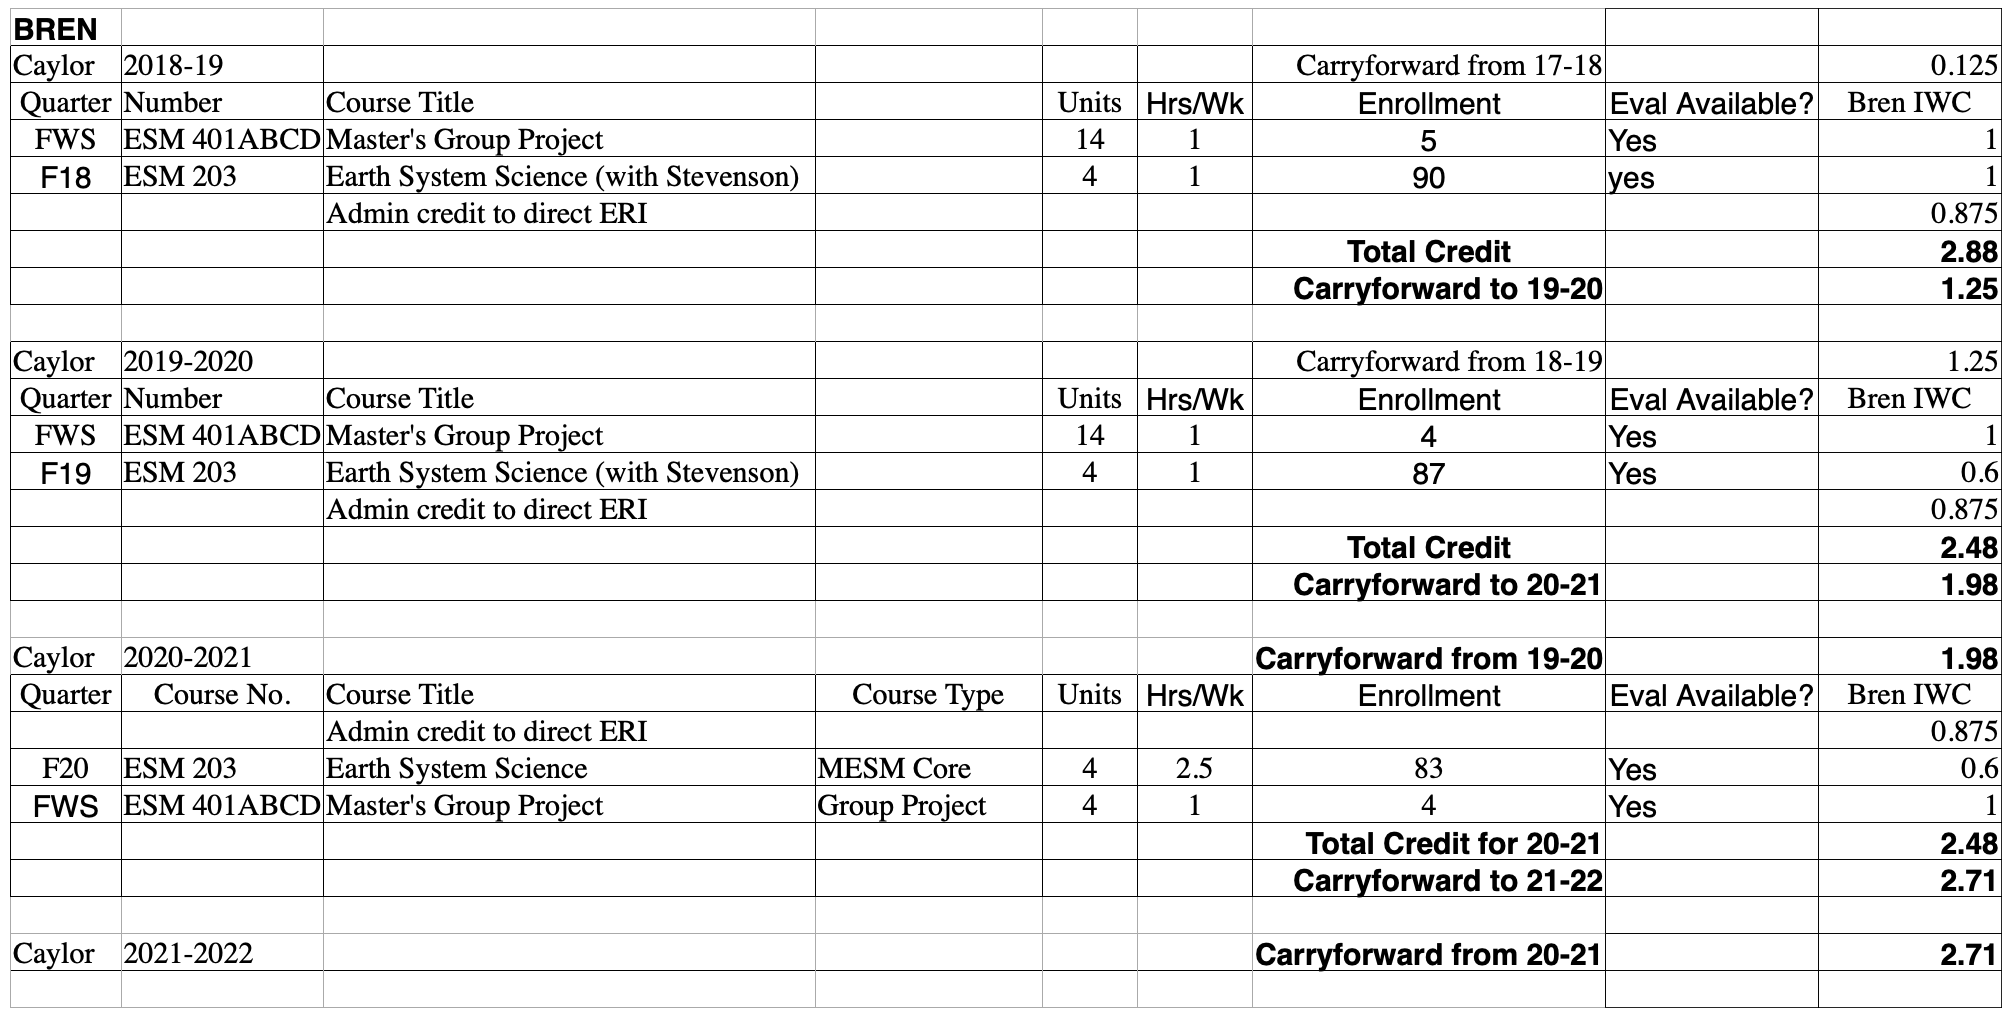
\includegraphics{bren_detailed_iwc.png}}
\end{centering}
}

\end{enumerate}

\vspace{0.5cm}
{\bf Catalog Courses:}
%\vspace{0.15cm}
% UC Bio-bib Catalog Courses Table
% Created on 2021-09-22 18:29

\begin{longtable}{p{1cm}p{7cm}p{0.75cm}rrrp{2.5cm}}
Qtr & Course & Class Type & Units & Hrs/Wk & Enrollment & ESCI/Written Evals Avail.\\
\hline 
\endfirsthead

\multicolumn{7}{c}%
{{Catalog Courses - continued from previous page }} \\ \\
Qtr & Course & Class Type & Units & Hrs/Wk & Enrollment & ESCI/Written Evals Avail.\\
\hline 
\endhead

\\
\multicolumn{7}{c}%
{{ Catalog Courses continued on next page }} \\
\endfoot

\hline \hline
\endlastfoot


F18 & GEOG 596, Directed Reading and Research & Tut &  & 2 & 2 & No/No    \\ 
F18 & ESM 203, Earth System Science & Lec & 4.0 & 1 & 90 & Yes/Yes  \href{https://ucsb.box.com/s/vvhpxerul6hbzum3fvmwigzd3y8yset6}{[link]}  \\ 
F18 & ESM 401B, Group Project - B & Dis & 4.0 & 1 & 5 & No/No    \\ 
F18 & GEOG 199RA, Independent Research Assistant & Tut &  & 1 & 1 & No/No    \\ 
F18 & GEOG 598, Master’s Thesis & Tut &  & 1 & 1 & No/No    \\ 
F18 & GEOG 599, PhD Dissertation & Tut &  & 2 & 2 & No/No    \\ 
W19 & GEOG 596, Directed Reading and Research & Tut &  & 1 & 1 & No/No    \\ 
W19 & ESM 401C , Group Project - C & Dis & 4.0 & 1 & 5 & No/No    \\ 
W19 & GEOG 599, PhD Dissertation & Tut &  & 2 & 2 & No/No    \\ 
S19 & GEOG 596, Directed Reading and Research & Tut &  & 1 & 1 & No/No    \\ 
S19 & ESM 401A, Group Project - A & Lec & 4.0 & 1 & 5 & No/No    \\ 
S19 & ESM 401D, Group Project - D & Dis & 2.0 & 1 & 4 & No/No    \\ 
S19 & GEOG 599, PhD Dissertation & Tut &  & 2 & 2 & No/No    \\ 
S19 & G136, Water, Energy, and Ecosystems & Lec & 4.0 & 1 & 10 & Yes/Yes  \href{https://ucsb.box.com/s/9oj1uqebr0a3gcg9brhfxw6ys8atw9oi}{[link]}  \\ 
F19 & GEOG 596, Directed Reading and Research & Tut &  & 4 & 4 & No/No    \\ 
F19 & ESM 203, Earth System Science & Lec & 4.0 & 1 & 87 & Yes/Yes  \href{https://ucsb.box.com/s/btln348spk7zsculb0swyrqe6nt0so33}{[link]}  \\ 
F19 & ESM 401B, Group Project - B & Dis & 4.0 & 1 & 4 & No/No    \\ 
F19 & GEOG 597, Individual Study - PhD Exam & Tut &  & 1 & 1 & No/No    \\ 
F19 & GEOG 598, Master’s Thesis & Tut &  & 1 & 1 & No/No    \\ 
F19 & GEOG 599, PhD Dissertation & Tut &  & 2 & 2 & No/No    \\ 
W20 & GEOG 596, Directed Reading and Research & Tut &  & 3 & 3 & No/No    \\ 
W20 & ESM 401C , Group Project - C & Dis & 4.0 & 1 & 4 & No/No    \\ 
W20 & GEOG 199, Independent Studies & Tut &  & 1 & 1 & No/No    \\ 
W20 & GEOG 599, PhD Dissertation & Tut &  & 2 & 2 & No/No    \\ 
S20 & GEOG 596, Directed Reading and Research & Tut &  & 1 & 1 & No/No    \\ 
S20 & ESM 401A, Group Project - A & Lec & 4.0 & 1 & 4 & No/No    \\ 
S20 & ESM 401D, Group Project - D & Dis & 2.0 & 1 & 4 & No/No    \\ 
S20 & GEOG 597, Individual Study - PhD Exam & Tut &  & 1 & 1 & No/No    \\ 
S20 & GEOG 598, Master’s Thesis & Tut &  & 1 & 1 & No/No    \\ 
S20 & GEOG 599, PhD Dissertation & Tut &  & 1 & 1 & No/No    \\ 
S20 & GEOG 136, Water, Energy, and Ecosystems & Lec & 4.0 & 1 & 10 & Yes/Yes  \href{https://ucsb.box.com/s/4k3squfamwz4gg5mj2q79wo5qk29bubb}{[link]}  \\ 
F20 & ESM 203, Earth System Science & Lec & 4.0 & 1 & 83 & Yes/Yes  \href{https://ucsb.box.com/s/x8g8gcl7mtfahclm1zledaita1z5tgin}{[link]}  \\ 
F20 & GEOG 596, Directed Reading and Research & Tut &  & 2 & 2 & No/No    \\ 
F20 & ESM 401B, Group Project - B & Dis & 4.0 & 1 & 4 & No/No    \\ 
F20 & GEOG 597, Individual Study - PhD Exam & Tut &  & 1 & 1 & No/No    \\ 
F20 & GEOG 598, Master’s Thesis & Tut &  & 1 & 1 & No/No    \\ 
F20 & GEOG 599, PhD Dissertation & Tut &  & 2 & 2 & No/No    \\ 
W21 & GEOG 596, Directed Reading and Research & Tut &  & 2 & 2 & No/No    \\ 
W21 & ESM 401C , Group Project - C & Dis & 4.0 & 1 & 4 & No/No    \\ 
W21 & GEOG 597, Individual Study - PhD Exam & Tut &  & 1 & 1 & No/No    \\ 
W21 & GEOG 598, Master’s Thesis & Tut &  & 1 & 1 & No/No    \\ 
W21 & GEOG 599, PhD Dissertation & Tut &  & 2 & 2 & No/No    \\ 
S21 & GEOG 596, Directed Reading and Research & Tut &  & 1 & 1 & No/No    \\ 
S21 & ESM 401A, Group Project - A & Lec & 4.0 & 1 & 5 & No/No    \\ 
S21 & ESM 401D, Group Project - D & Dis & 2.0 & 1 & 4 & No/No    \\ 
S21 & GEOG 597, Individual Study - PhD Exam & Tut &  & 1 & 1 & No/No    \\ 
S21 & GEOG 598, Master’s Thesis & Tut &  & 1 & 1 & No/No    \\ 
S21 & GEOG 599, PhD Dissertation & Tut &  & 1 & 1 & No/No    \\ 
S21 & GEOG 288KC, Special Topics in Geography & Dis & 2.0 & 1 & 5 & Yes/Yes  \href{https://ucsb.box.com/s/wkdexakrybpri16xk2gu5860so2ae0xa}{[link]}  \\ 
 
\end{longtable}



\vspace{0.5cm}
{\bf MESM Projects Advised}
%\vspace{0.15cm}
% UC Bio-bib MESM Projects Table
% Created on 2021-08-20 17:50

\begin{longtable}{p{1cm}p{2.5cm}p{3cm}p{2cm}p{2cm}p{2cm}p{2cm}}
Year & Project Title & Students & Q3 & Q4 & Q5 & Q7\\
\hline 
\endhead 
2020 - 2021 & Wild Pig Management at the Jack and Laura Dangermond Preserve & Peter Omasta, Shuhan Song, Benson Truong, AJ Zekanoski & 100\% Strongly Agree & 100\% Excellent & 100\% Always & 100\% Excellent \\ 
2019 - 2020 & A stormwater management plan to reduce pollution in Maunalua Bay & Eleonore Durand, Natalie Dornan, Tara Jagadish, Erica Johnson & 0\% Strongly Agree, 100\% Somewhat Agree & 50\% Satisfactory, 50\% Fair & 75\% Always, 25\% Usually & 75\% Satisfactory, 25\% Poor \\ 
2018 - 2019 & The Dangermond Preserve: Integrating historical chance and future projections to guide conservation & Brad Anderson, Mechan Bowen, Lucy Genua, Kam Howo, Genelle Ives & 40\% Somewhat agree, 40\% Neutral, 20\% Somewhat disagree & 20\% Very Good, 60\% Satisfactory, 20\% Fair & 40\% Usually, 20\% Sometimes, 40\% Rarely & 20\% Very good, 60\% Satisfactory, 20\% Fair \\ 
\end{longtable}



\vspace{1cm}
{\bf Undergraduate Projects Directed:}
% UC Bio-bib Catalog UndergradAdvising Table
% Created on 2019-02-20 10:20

\begin{longtable}{lp{6.5cm} p{4.5cm}p{2cm}p{4cm}}
Student & Project & Role & Year \\
\hline 
\endfirsthead


\multicolumn{4}{c}%
{{Undergraduate Projects Directed - continued from previous page }} \\ \\
Student & Project & Role & Year \\
\hline 
\endhead

\\
\multicolumn{4}{c}%
{{ Undergraduate Projects Directed continued on next page }} \\
\endfoot

\hline \hline
\endlastfoot

Sierra Yarnes & Hydrological dynamics of the Dangermond Preserve & Chair & 2020 \\
\end{longtable}


%{\setlength{\extrarowheight}{3.5pt}
%\tablehead{}
%\begin{supertabular}{lp{11cm}cc} 
%Student & Project & Chair/ & Yr Deg \\
% & & Member & Compl. \\
% \hline
%%Madison Gray & History of Urban Design in Edinburgh & Chair &  2008 \\
%%Eric Wilder & An assessment of environmental planning in Humboldt County, CA & Chair & 2010 \\ 
%\end{supertabular}
%}
%None.
\newpage
\vspace{1cm}
{\bf Graduate Degree Committees, MA/MS Committees:}
\vspace{0.25cm}
% UC Bio-bib Catalog GraduateAdvising Table
% Created on 2019-02-20 10:20

\begin{longtable}{lp{1.5cm} p{2cm}p{2.5cm}p{6.5cm}}

Student & Year & Institution & Chair/Member & Current Employment\\
\hline 
\endfirsthead

\multicolumn{5}{c}%
{{Graduate Degree Committees, MA/MS Committees - continued from previous page }} \\ \\
Student & Year & Institution & Chair/Member & Current Employment\\
\hline 
\endhead

\\
\multicolumn{5}{c}%
{{ Graduate Degree Committees, MA/MS Committees continued on next page }} \\
\endfoot

\hline \hline
\endlastfoot

Ryan Avery & 2020 & UCSB & Chair & Analyst  -  Development Seed \\
\end{longtable}




\vspace{0.5cm}
{\bf Graduate Degree Committees, Ph.D. Committees:}
\vspace{0.25cm}
% UC Bio-bib Catalog GraduateAdvising Table
% Created on 2018-09-24 17:41

\tablehead{Student & Year & Instituion & Chair/Member & Current Employment\\ \hline}
\begin{supertabular}{lp{1.5cm} p{3.5cm}p{2cm}p{4.5cm}}
Cynthia Gerlein-Safdi & 2017 & Princeton University, Civil \& Environmental Engineering & Chair & Postdoctoral Researcher - University of Michigan\\
Stephanie Debats & 2017 & Princeton University, Civil \& Environmental Engineering & Chair & Autonomy Engineer - Uber\\
Cascade Tuholske & In Progress & UCSB, Geography & Chair &  - \\
Drew Gower & In Progress & Princeton University, Civil \& Environmental Engineering & Chair &  - \\
Keita DeCarlo & In Progress & Princeton University, Civil \& Environmental Engineering & Chair &  - \\
Natasha Krell & In Progress & UCSB, Geography & Chair &  - \\
Ryan Avery & In Progress & UCSB, Geography & Chair &  - \\
Chris Heckman & In Progress & UCSB, Bren & Committee Member &  - \\
Elizabeth Forbes & In Progress & UCSB, Ecology, Evolution, and Marine Ecology & Committee Member &  - \\
Fernanda Riberio & In Progress & UCSB, Geography & Committee Member &  - \\
Mike Johnson & In Progress & UCSB, Geography & Committee Member &  - \\
Sara Lafia & In Progress & UCSB, Geography & Committee Member &  - \\
Susan Meerdink & In Progress & UCSB, Geography & Committee Member &  - \\
\end{supertabular}




\vspace{0.5cm}
{\bf Postdoctoral Scholars Supervised:}
%\vspace{0.25cm}
% UC Bio-bib Catalog Postdoctoral Advising Table
% Created on 2018-06-30 11:26

\tablehead{Postdoctoral Researcher & Years & Affiliation & Current Employment\\ \hline}
\begin{supertabular}{lp{1.5cm} p{3.5cm}p{4.5cm}}
Marc Mayes & 2016 -  & UCSB, Geography &   - \\
\end{supertabular}



\vspace{0.5cm}
{\bf Other Teaching Contributions:}
\vspace{0.25cm}

Instructor, Coupled Natural-Human Systems Short Course. University of California, Irvine. August, 2018
Advisor, WAVES Lab High School Summer Internship, Mahima Agarwal, Palo Alto, CA. June, 2018
 
%{\setlength{\extrarowheight}{3.5pt}
%\tablehead{}
%\begin{supertabular}{cp{16cm}} 
%- & Coordinator and instructor for the UCSB Spatial Perspectives on Curriculum Enhancement (SPACE) workshop, July 2007 \\
%- & Took the Geography 20 honors section on a field trip to UC San Diego to attend the Surfing, Arts, Sciences, and Issues Conference at Scripps Institute, February 2007 \\
%- & Mentor/advisor for Sam Boysel (San Marcos High School student) for his senior honors science project. \\
%- & Faculty undergraduate advisor, 2008-09, Geography \\
%\end{supertabular}
%}
%\newpage

\vspace{0.5cm}
\textbf{PART III.  PROFESSIONAL ACTIVITIES}

\vspace{0.5cm}
\textbf{Lectures and Seminars Presented:}
\vspace{0.25cm}
{\setlength{\extrarowheight}{3.5pt}
% UC Bio-bib Lectures Table
% Created on 2021-06-04 12:23

\begin{longtable}{lp{10.0cm}p{4.5cm}}
Month/Year & Title & Meeting/Place\\
\hline 
\endhead 
8/2018 & Invited Speaker, Session on ``Vegetation dynamics and ecosystem resilience under global climate change'', Ecological Society of America Annual Meeting & New Orleans, LA \\
8/2018 & Instructor, Coupled Natural-Human Systems Short Course & University of California, Irvine \\
5/2019 & Keynote Speaker, Board of Trustees Meeting & University of California, Santa Barbara \\
8/2019 & Invited Speaker, 44th New Phytologist Symposium & Accra, Ghana \\
9/2019 & Invited Speaker, Department of Civil and Environmental Engineering & University of Florida \\
12/2019 & Invited Speaker, Fall Meeting, American Geophysical Union & San Francisco, CA \\
12/2020 & Invited Speaker, Fall Meeting, American Geophysical Union & San Francisco, CA \\
5/2021 & Keynote Speaker, AI and ML in Earth \& Environmental Science & Helmholtz Institute \\
\end{longtable}


}


\vspace{0.5cm}
\textbf{Conference Posters and Presentations:}
\vspace{0.25cm}
{\setlength{\extrarowheight}{3.5pt}
% UC Bio-bib Proceedings Table
% Created on 2018-10-17 21:09

\begin{longtable}{lp{10.0cm}p{4.5cm}}
Month/Year & Title & Meeting/Place\\
\hline 
\endhead 
 12/2016 & {\bf Assessment of SMAP L2/L3 Soil Moisture Products using In Situ Based Core Validation Sites}. Colliander, A and Jackson, TJ and Bindlish, R and Chan, S and Das, NN and Kim, S and Cosh, MH and Dunbar, RS and Asanuma, J and Aida, K and others  & American Geophysical Union Fall Meeting\\
 12/2016 & {\bf Linking Carbon Flux Dynamics and Soil Structure in Dryland Soils}. DeCarlo, Keita F and Caylor, Kelly K  & American Geophysical Union Fall Meeting\\
 12/2016 & {\bf Characterization of canopy dew formation in tropical forests using active microwave remote sensing}. Gerlein-Safdi, C and Frolking, SE and Caylor, K.K.  & American Geophysical Union Fall Meeting\\
 12/2016 & {\bf An ecohydrologic framework for simulating catchment constraints on smallholder irrigation systems in drylands}. Gower, D and McCord, PF and Caylor, K.K. and Dell'Angelo, J and Evans, TP  & American Geophysical Union Fall Meeting\\
 12/2016 & {\bf Harmonizing Social and Environmental Dynamics in Earth Systems Modeling}. Evans, Tom P and Estes, Lyndon D and Caylor, Kelly K and McCord, Paul Frederick and Gower, Drew and Konar, M and Baylis, K and Waldman, K and Blekking, J and Schlachter, T  & American Geophysical Union Fall Meeting\\
 12/2016 & {\bf Combining Human and Machine Learning to Map Cropland in the 21st Century's Major Agricultural Frontier}. Estes, Lyndon D and Debats, SR and Caylor, Kelly K and Evans, Tom P and Gower, Drew and McRitchie, Dennis and Searchinger, Timothy and Thompson, David R and Wood, Eric F and Zeng, Lindy  & American Geophysical Union Fall Meeting\\
 12/2016 & {\bf Rapid Monitoring of Drought Impacts on Small-Scale Farms in Africa through Integration of Farmer SMS data and Environmental Sensors}. Evans, Tom P and Caylor, Kelly K and Estes, Lyndon D and Plale, Beth A and Attari, Shahzeen and Waldman, Kurt  & American Geophysical Union Fall Meeting\\
 12/2016 & {\bf Using Small Drone (UAS) Imagery to Bridge the Gap Between Field-and Satellite-Based Measurements of Vegetation Structure and Change}. Mayes, MT and Estes, LD and Gago, X and Debats, SR and Caylor, K.K. and Manfreda, S and Oudemans, P and Ciraolo, G and Maltese, A and Nadal, M and others  & American Geophysical Union Fall Meeting\\
 12/2016 & {\bf Can we forecast farmers' yields? The relationships between rainfall variability, farmers' expectations, and actual yields in a tropical dryland}. Zeng, Z and Tian, D and Estes, LD and Evans, TP and Wood, EF and Caylor, K.K.  & American Geophysical Union Fall Meeting\\
 4/2017 & {\bf Dryland feedbacks between biogeochemistry, plants, and surface hydrological dynamics}. K.K. Caylor (INVITED) & Association for the Sciences of Limnology and Oceanography\\
 12/2017 & {\bf High spatial resolution mapping of land cover types in a priority area for conservation in the Brazilian savanna}. Ribeiro, F and Roberts, DA and Hess, LL and Davis, FW and Caylor, K.K. and Nackoney, J and Antunes Daldegan, G  & American Geophysical Union Fall Meeting\\
 12/2017 & {\bf Simulating the impact of water storage on agricultural intensification and deforestation in Northern Thailand}. Gower, D and Zeng, Z and Caylor, K.K. and Wood, EF  & American Geophysical Union Fall Meeting\\
 12/2017 & {\bf Effects of dew deposition on transpiration and carbon uptake in leaves}. Gerlein-Safdi, C and Koohafkan, M and Chung, M and Rockwell, FE and Thompson, SE and Caylor, K.K.  & American Geophysical Union Fall Meeting\\
 12/2017 & {\bf Is deciduousness a key to climate resilience among iconic California savanna oak species? Relating phenological habits to seasonal indicators of tree physiological and water stress across field, hyperspectral, drone (UAS)-based multispectral and thermal image data}. Mayes, MT and Caylor, K.K. and Ehlmann, BL and Greenberger, RN and Estes, LD  & American Geophysical Union Fall Meeting\\
 12/2017 & {\bf Real-time monitoring of smallholder farmer responses to intra-seasonal climate variability in central Kenya}. Krell, N and Evans, TP and Estes, LD and Caylor, K.K.  & American Geophysical Union Fall Meeting\\
 4/2018 & {\bf On the use of unmanned aerial systems for environmental monitoring}. Manfreda, S., Ben Dor, E., Caylor, K.K., Ciraolo, G., De Lima, I., De Lima, J.L.M., Estes, L., Frances, F., Helman, D., Kohv, M., Lucas, R., Madrigal, V.P., Mallinis, G., Maltese, A., McCabe, M., Miller, P., Perks, M., Ruiz-Perez, G., Tauro, F., Toth, B.  & European Geosciences Union, General Assembly 
\\
 4/2018 & {\bf Integrating humans and machines to map smallholder-dominated agricultural frontiers}. Estes, L., Caylor, K.K., Debats, S., Eastman, R., Thompson, D.R.   & Association of American Geographers Annual Meeting\\
 4/2018 & {\bf Towards assessing urban food security and nutrition in West Africa}. Tuholske, C., Andam, K., Blekking, J., Caylor, K., Evans, T.  & American Association of Geographers Annual Meeting \\
 8/2018 & {\bf Multi-scale dynamics of vegetation responses to changing rainfall variability in dryland regions}. K.K. Caylor (INVITED) & Ecological Society of America\\
\end{longtable}


}

%\newpage
\vspace{0.5cm}
\textbf{Grants and Contracts:}
\vspace{0.25cm}
{\setlength{\extrarowheight}{3.5pt}
% UC Bio-bib Funding Table
% Created on 2021-05-21 10:00

\begin{longtable}{p{1.75cm}>{\raggedright}p{2.75cm}p{5.5cm}p{1cm}p{1.25cm}p{1.25cm}p{1cm}}
Year & Source & Title & Role & Amount & Personal Share & New/Cont.\\
\hline 
\endhead 
\end{longtable}


}

\vspace{0.5cm}
\textbf{Reviewing and Refereeing Activity:}
\vspace{0.2cm}
% UC Bio-bib Reveiwer Activity Table
% Created on 2018-06-29 08:27

\tablehead{Year & Activity & Journal/Agency\\ \hline}
\begin{supertabular}{llp{12cm}}
2016 & Referee & Environmental Research Letters   \\
2016 & Referee & Geophysical Research Letters  (2) \\
2016 & Referee & NSF Hydrological Sciences   \\
2017 & Program Director & Earth Research Institute Graduate Fellowship Program   \\
2017 & Referee & Earth and Space Science   \\
2017 & Referee & Environmental Research Letters  (4) \\
2017 & Referee & Geophysical Research Letters   \\
2017 & Referee & Nature Communications   \\
2017 & Referee & Water Resources Research   \\
2017 & Tenure case reviewer & Indiana University   \\
2017 & Tenure case reviewer & University of Alabama   \\
2017 & Tenure case reviewer & University of Cape Town   \\
2018 & Program Director & Earth Research Institute Graduate Fellowship Program   \\
2018 & Promotion case reviewer & University of Texas, Austin   \\
2018 & Referee & Agricultural and Forest Meteorology   \\
2018 & Referee & Environmental Research Letters  (2) \\
2018 & Referee & Global and Planetary Change   \\
2018 & Referee & JGR Biogeosciences   \\
2018 & Referee & Journal of Water Resources Planning \& Management   \\
2018 & Referee & Mountain Research and Development    \\
2018 & Referee & NSF Hydrological Sciences   \\
2018 & Referee & Nature Climate Change   \\
2018 & Referee & PLOS One  (2) \\
\end{supertabular}



\vspace{0.25cm}
\textbf{Special Appointments:}
\vspace{0.15cm}
% UC Bio-bib Special Appointments Table
% Created on 2021-08-23 10:41

\begin{longtable}{llp{12cm}}
Year & Role & Organization\\
\hline 
\endhead 
2015 - 2019 & Member & Editorial Board, Environmental Research Reviews, Environmental Research Letters \\
2020  & Editor & Earth's Future, American Geophysical Union \\
2021 & Editor & Earth's Future, American Geophysical Union \\
\end{longtable}


\newpage

\vspace{0.2cm}
\textbf{Other Professional Activities:}
\vspace{0.15cm}
% UC Bio-bib Other Professional Activities Table
% Created on 2022-01-19 10:54

\begin{longtable}{llp{12cm}}
Year & Role & Organization\\
\hline 
\endfirsthead


\multicolumn{3}{c}%
{{None - continued from previous page }} \\ \\
Year & Role & Organization\\
\hline 
\endhead

\\
\multicolumn{3}{c}%
{{ None continued on next page }} \\
\endfoot

\hline \hline
\endlastfoot

2018 & Tenure case reviewer & University of Toronto \\
2018 & Promotion case reviewer & SUNY-ESF \\
2018 & Promotion case reviewer & University of Washington \\
2018 & Co-Convenor & AGU Fall Meeting, Session on ``Indicators of Plant Water Availability and Stress in Drought-Prone Forests at a Range of Spatial and Temporal Scales'' \\
2020 & Promotion case reviewer & Texas A\&M University \\
2021 & Tenure case reviewer & Michigan State University \\
2021 & Tenure case reviewer & Duke University \\
\end{longtable}



%\newpage

\vspace{0.25cm}
\textbf{PART IV.  SERVICE}

\vspace{0.5cm}
\textbf{University Service:}
\vspace{0.2cm}
% UC Bio-bib Professional Generic Service Table
% Created on 2021-08-23 10:41

\begin{longtable}{llp{12cm}}
Year & Role & Service\\
\hline 
\endhead 
2018 - 2019 & Participating Faculty & Interdepartmental PhD Emphasis in Environment and Society \\
2018 - 2019 & Member & Data Science Curriculum Committee \\
2018 - 2019 & Member & North Campus Open Space Administrative Advisory Group \\
2018 - 2019 & Member & Campus Data Science Initiative Working Group \\
2018 - 2019 & Member & Data Science Working Group, UCSB \\
2018 - 2019 & Ex-Officio Member & Earth Research Institute Advisory Committee, UCSB \\
2018 - 2019 & Director & Earth Research Institute, University of California, Santa Barbara \\
2018 - 2019 & Chair & Earth Research Institute, Personnel Committee \\
2018 - 2019 & Member  & NCEAS Campus Advisory Committee  \\
2019 - 2020 & Participating Faculty & Interdepartmental PhD Emphasis in Environment and Society \\
2019 - 2020 & Member & Data Science Curriculum Committee \\
2019 - 2020 & Member & Campus Data Science Initiative Working Group \\
2019 - 2020 & Member & North Campus Open Space Administrative Advisory Group \\
2019 - 2020 & Member & Dangermond Endowed Chair Search Committee, Office of Research \\
2019 - 2020 & Ex-Officio Member & Earth Research Institute Advisory Committee, UCSB \\
2019 - 2020 & Chair & Earth Research Institute, Personnel Committee \\
2019 - 2020 & Member & Space Committee, Office of Research \\
2020 - 2021 & Participating Faculty & Interdepartmental PhD Emphasis in Environment and Society \\
2020 - 2021 & Member & Offsite Research Committee, University of California, Santa Barbara \\
2020 - 2021 & Member & Campus Data Science Initiative Working Group \\
2020 - 2021 & Member & Steering Committee, Climate Hazards Center, UCSB \\
2020 - 2021 & Member & North Campus Open Space Administrative Advisory Group \\
2020 - 2021 & Ex-Officio Member & Earth Research Institute Advisory Committee, UCSB \\
2020 - 2021 & Ex-Officio Member & Earth Research Institute Computing Committee, UCSB \\
2020 - 2021 & Chair & NCEAS Campus Advisory Committee  \\
2020 - 2021 & Chair & Earth Research Institute, Personnel Committee \\
\end{longtable}



\vspace{0.25cm}
\textbf{Department Service:}
\vspace{0.2cm}
% UC Bio-bib Professional Generic Service Table
% Created on 2021-08-20 17:50

\begin{longtable}{llp{12cm}}
Year & Role & Service\\
\hline 
\endhead 
2018 - 2019 & Member  & Sustainable Water Markets (SWM) Fellowship Program Committee, Bren School of Environmental Science and Management, University of California, Santa Barbara \\
2018 - 2019 & Chair & Space Committee, Department of Geography, University of California, Santa Barbara \\
2018 - 2019 & Member & Graduate Admission Committee, Department of Geography, University of California, Santa Barbara \\
2018 - 2019 & Member & Vegetation Data Science Faculty Search Committee, Department of Geography, UCSB \\
2019 - 2020 & Chair & Space Committee, Department of Geography, University of California, Santa Barbara \\
2019 - 2020 & Member & Group Project Committee, Bren School of Environmental Science and Management, University of California, Santa Barbara \\
2019 - 2020 & Member & Dangermond Endowed Chair Search Committee, Department of Geography \\
2019 - 2020 & Member  & Sustainable Water Markets (SWM) Fellowship Program Committee, Bren School of Environmental Science and Management, University of California, Santa Barbara \\
2020 - 2021 & Chair & Space Committee, Department of Geography, University of California, Santa Barbara \\
2020 - 2021 & Member & DEI Committee, Department of Geography, UCSB \\
2020 - 2021 & Member & Faculty Executive Committee, Bren School of Environmental Science and Management, University of California, Santa Barbara \\
\end{longtable}



\vspace{1.25cm}
\textbf{Public Service:}
\vspace{0.2cm}
None Provided.



\end{document}





